\documentclass[11pt,a4paper]{report}

% Aberstwyth dissertation LaTeX Template
% Authors: Dr. Hannah Dee (hmd1@aber.ac.uk), Neil Taylor (nst@aber.ac.uk)
% This has been adapted from the Leeds Thesis template and the 
% Group Project template for Computer Science in Aberystywth University.
% 
% All comments and suggestions welcome.
%
% Template designed to be used with pdflatex: it may need alteration to
% run with a different LaTeX engine

% To build document on the unix command line, run four commands:
 
% pdflatex dissertation
% bibtex dissertation
% pdflatex dissertation
% pdflatex dissertation

% you will end up with dissertation.pdf 
\usepackage{mmp}

% the following packages are used for citations - You only need to include one. 
%
% Use the cite package if you are using the numeric style (e.g. IEEEannot). 
% Use the natbib package if you are using the author-date style (e.g. authordate2annot). 
% Only use one of these and comment out the other one. 
\usepackage{cite}
%\usepackage{natbib}
\usepackage[acronym,toc]{glossaries}
\usepackage{caption}
\usepackage{subcaption}

% Use the following to selectively exclude chapters
%\includeonly{cover,abstract,acknowledge,declare,chapter1,chapter2}


\newacronym{rts}{RTS}{real-time strategy}



\begin{document}

% all of the include directives below refer to tex files
% so 
\title{MapWars: Location-Aware Multi-Player Mobile Game}

% Your name
\author{Luke Ward}

% Your email 
\authoremail{luw9@aber.ac.uk}

\degreeschemecode{G400} %e.g. G400 
\degreeschemetitle{Computer Science} % e.g. Computer Science
\degreetype{BSc}

\modulecode{CS39440} % i.e. CS39440, CC39440, CS39620
\moduletitle{Major Project} % i.e. Major Project or Minor Project

\date{25th March 2013} % i.e. the date of this version of the report

\status{Draft} % Use draft until you create the release version. Then, change this to Release.
\version{1.0}

%The title and name of your supervisor.
\supervisor{Dr./Prof. My Supervisor} 

%The email for your supervisor. 
\supervisoremail{rzz@aber.ac.uk}

\maketitle



 includes cover.tex - to change the content,
% edit the tex file

\pagenumbering{roman}

% This is the front page

\title{MapWars: Location-Aware Multi-Player Mobile Game}

% Your name
\author{Luke Ward}

% Your email 
\authoremail{luw9@aber.ac.uk}

\degreeschemecode{G400} %e.g. G400 
\degreeschemetitle{Computer Science} % e.g. Computer Science
\degreetype{BSc}

\modulecode{CS39440} % i.e. CS39440, CC39440, CS39620
\moduletitle{Major Project} % i.e. Major Project or Minor Project

\date{25th March 2013} % i.e. the date of this version of the report

\status{Draft} % Use draft until you create the release version. Then, change this to Release.
\version{1.0}

%The title and name of your supervisor.
\supervisor{Dr./Prof. My Supervisor} 

%The email for your supervisor. 
\supervisoremail{rzz@aber.ac.uk}

\maketitle



                        

% Set up page numbering
\pagestyle{empty}

% declarations of originality 
\thispagestyle{empty}

%%%
%%% You must sign the declaration of originality. 
%%%
\begin{center}
    {\LARGE\bf Declaration of originality}
\end{center}

In signing below, I confirm that:

\begin{itemize}
\item{This submission is my own work, except where clearly
indicated.  }

\item{I understand that there are severe penalties for plagiarism 
and other unfair practice, which can lead to loss of marks
or even the withholding of a degree. }
 
\item{I have read the sections on unfair practice in the Students' 
Examinations Handbook and the relevant sections of the 
current Student Handbook of the Department of Computer 
Science.}
 
\item{I understand and agree to abide by the University's
regulations governing these issues.}
\end{itemize}

\vspace{3em}
Signature ............................................................  \\

\vspace{1em}
Date ............................................................ \\

%%% 
%%% We would like to make a selection of final reports available to students that take 
%%% this module in future years. To enable us to do this, we require your consent. You 
%%% are not required that you do this, but if you do give your consent, then we will have 
%%% the option to select yours as one of a number of reports as examples for other 
%%% students. If you would like to give your consent, then please include the following 
%%% text and sign below. If you do not wish to give your consent, please remove this 
%%% from your report. 
%%%
\vspace{5em}
\begin{center}
    {\LARGE\bf Consent to share this work}
\end{center}

In signing below, I hereby agree to this dissertation being made available to other
students and academic staff of the Aberystwyth Computer Science Department.  

\vspace{3em}
Signature ............................................................  \\

\vspace{1em}
Date ............................................................ \\

               

\thispagestyle{empty}

\begin{center}
    {\LARGE\bf Acknowledgements}
\end{center}

I am grateful to...

I'd like to thank...
 % Acknowledgements
\thispagestyle{empty}

\begin{center}
    {\LARGE\bf Abstract}
\end{center}

MapWars is the culmination of an investigation into the feasibility of creating a location-aware, multi-player \gls{rts} game for a mobile platform. Consideration about which platform to support is presented with the final decision being to focus on Google's Android operating system.

The game combines strategic game play against multiple players in a persistent environment, where game play is based on map of Earth and users are restricted in game to their real world location. Giving each user the capability to create their own army and battle against other players within their local area.

At the same time consideration was made to protect each users privacy and create a fair gaming experience. Thus different techniques on how to prevent crafted requests designed to circumnavigate limits placed in the Android client.

                 % Abstract

\pagenumbering{roman}
\pagestyle{fancy}
\fancyhead{}
\fancyfoot[C]{\thepage}
\renewcommand{\headrulewidth}{0 pt}
\renewcommand{\chaptermark}[1]{\markboth{#1}{}}

\tableofcontents   
\newpage
% \listoffigures
% \newpage 
% \listoftables
% \newpage

% Set up page numbering
\pagenumbering{arabic}

\setchapterheaderfooter

% include the chapters
\chapter{Background \& Ojectives}

\section{Background}
Real-time strategy (RTS) games have a huge market on desktop environments, but have yet to make the break through into the mobile gaming market. This is mostly attributed to the complex control mechanisms that need to be executed precisely. A mobile devices form factor restricts the number of controls that can be presented to the user at any given time as well as the precision in which these commands can be issued.

RTS games are generally designed around large, expansive maps that cover a large range of environments and landscapes. The game map shapes how the game will be played, how involved the player feels and ultimately the engagement of players. These maps can take years to develop and result in one of the largest costs within the development process. So when coming up with an environment why not take advantage of a ready made one? That of planet Earth.

Building a game where the game play takes place on a map of Earth has a number of benefits. First is the scale of a map covering 510 million square kilometres of varying terrain and features. This scale also contains a huge level of detail that could not be achieved by a team of designers. Along side this there is the feeling of familiarity, unlike when starting a new game and having to teach the player about the environment, the user will already have a well formed model in their own head. Along with highly detailed knowledge about certain areas especially those within close proximity of their current location.

Mobile devices have a whole host of unique features and sensors that set it apart from other gaming platforms. One feature that has been widely adopted in a huge range of different applications is location. A users location can be easily determined with a number of different components present on most modern smart phones, these are a GPS chip and the mobile GSM network. Although location has been used extensively in applications it has yet to be utilized effectively as a key metric within a game. This extra information about the user would enable a game set around the physical world to be able to be integrated with the user. Instead of placing new users randomly on a unfamiliar map they can be placed in their real location. Thus giving them a chance to use their own knowledge of their surroundings to help them within the game environment.


\section{Market}

A worldwide RTS game that combines a map of the world and data gathered about the user combine to create a unique gaming experience and could add an entirely new dimension to the genre. This can also reduce the learning curve and thus shorten the time between installation and engagement. With the sheer number of applications available on a mobile platform combined with the ease and minimal to no cost of installing new applications, this is important to reduce the chance of the user simply finding an alternative.

\subsection{Choosing a platform}
The current mobile platform oligopoly results in their only being two viable platforms, Apple's iOS and Google's Android OS. The Android operating system, as of February 2013, had over 51\% market share in the US\cite{smartphone_market}. Closely followed by the original and most established app ecosystem of Apple iOS. Even though there are other platforms, such as Windows phone and Blackberry, none of these have the market share allow them to be a primary platform of choice. Therefore choosing between the two platforms can be an important decision for mobile developers, both platforms offer their own unique advantages and disadvantages. Android on the one hand has the lead on market share offering a larger audience, although this will not directly affect engagement or return.

This years Developer Economics report\cite{de} looks at all aspects of the mobile app market and is an invaluable insight into both the market and consumer trends. As well as evaluating the current market it also gets feedback from developers as to their experiences with different platforms as well as their success.

\begin{figure}[H]
  \centering
   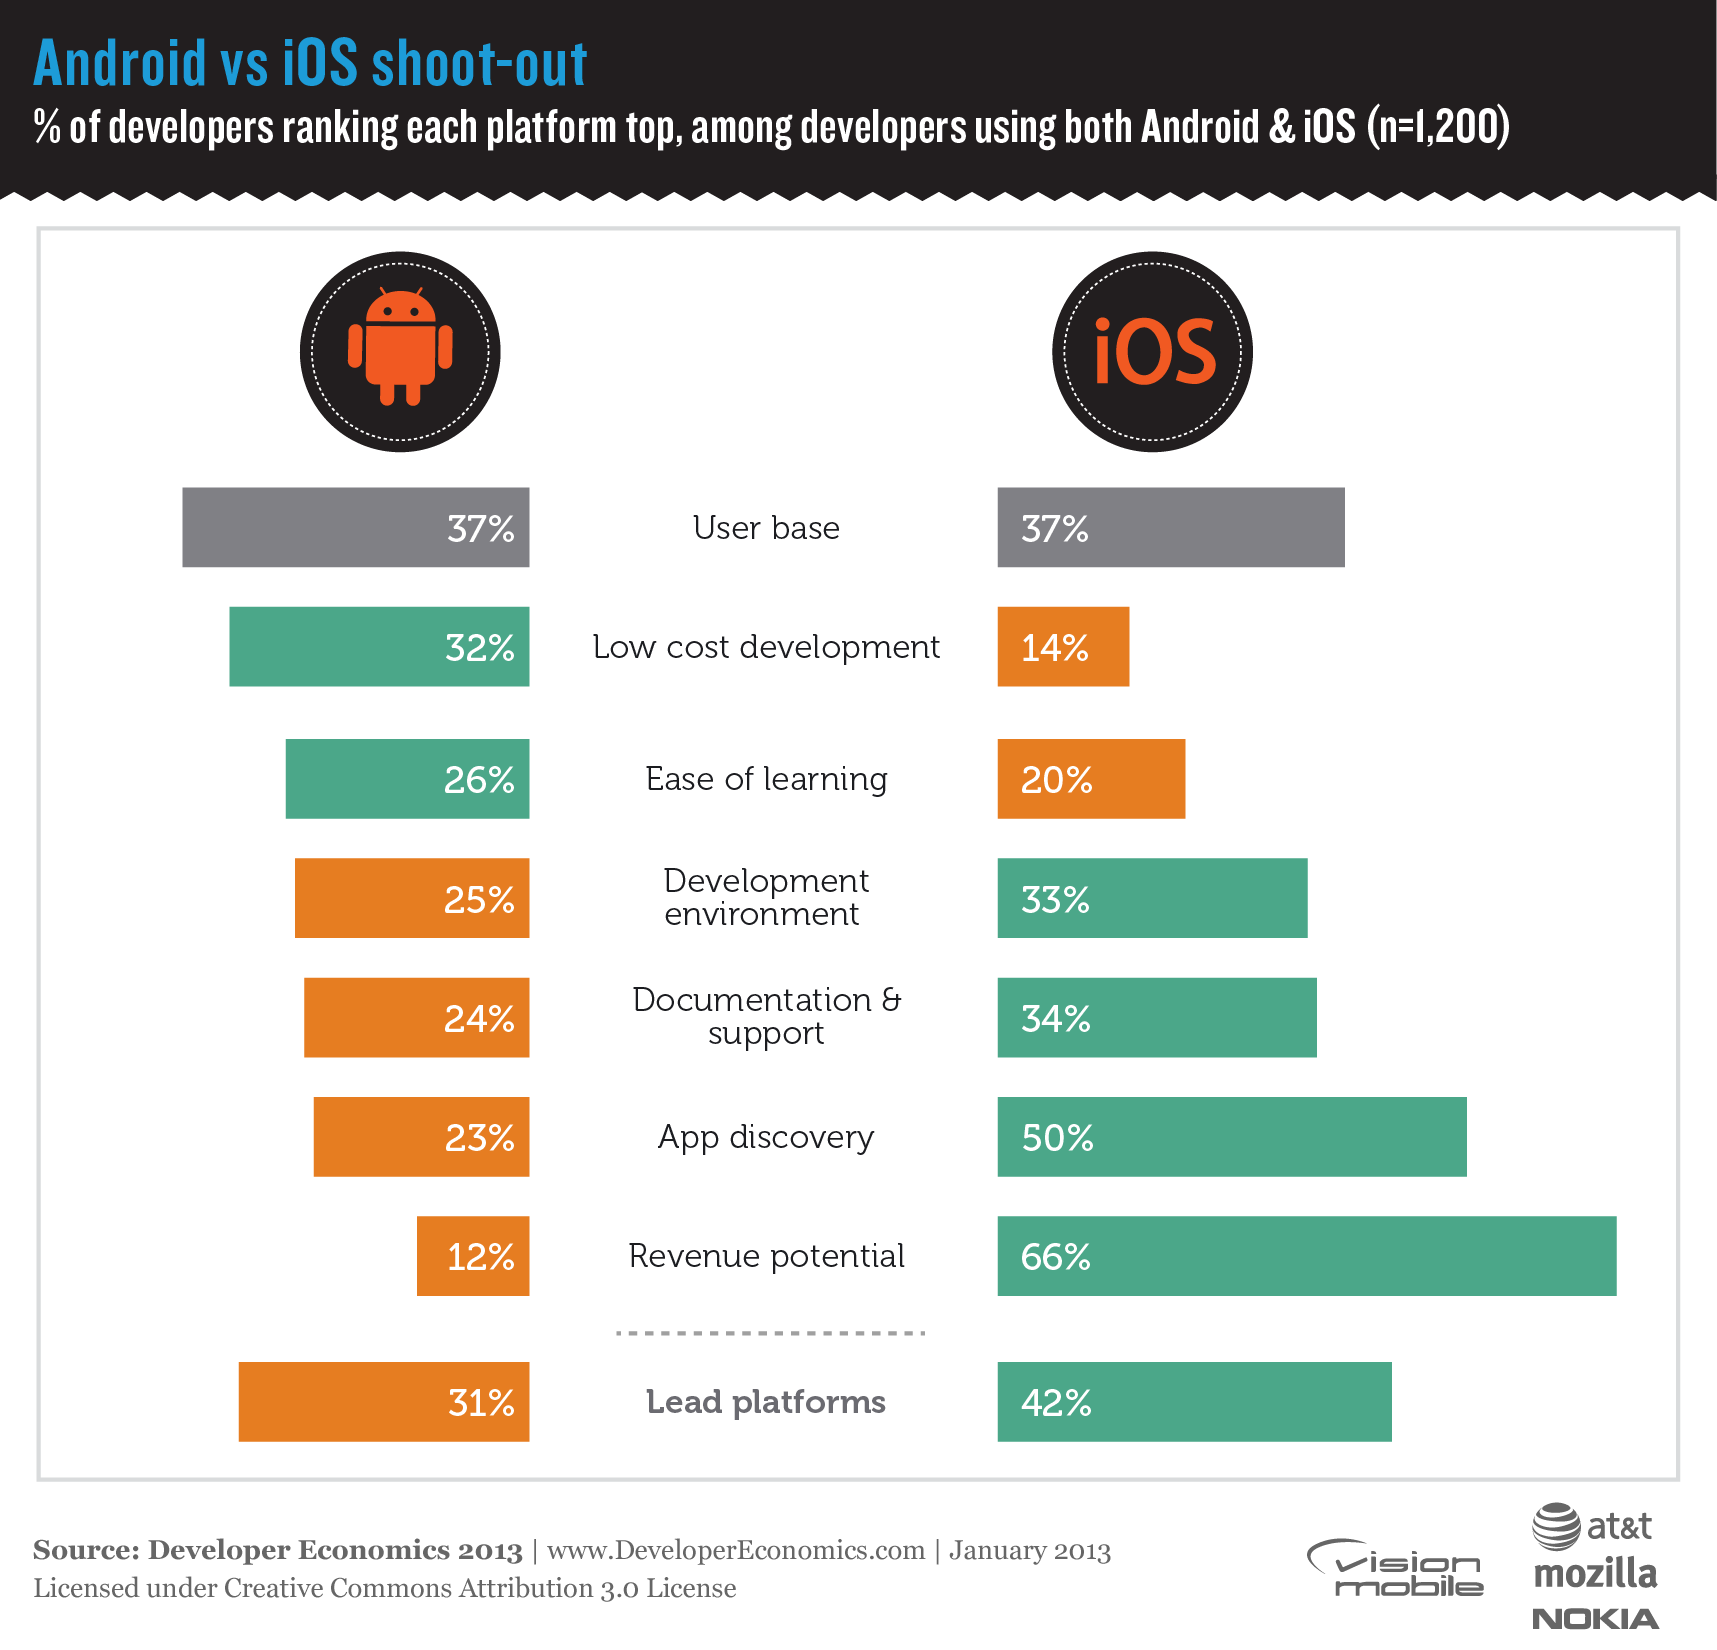
\includegraphics[width=0.8\textwidth]{Images/android_ios.png}
  \caption{Developer Economics report\cite{de} shows iOS\\as the leading platform among developers}
  \label{fig:de}
\end{figure}

As shown in Figure \ref{fig:de} iOS does indeed have a number of advantages over Android. Most importantly is the drastically increased chance of discovery as well as the expected return from applications on the iOS platform. For this project however less emphasis was placed on the success of the finished application and more on the process of creating it. Therefore the metrics of development cost and learning curve were considered to be more important. Aside from the Developer Economics findings there were a number of other more fundamental reasons as to why Android was the preferable platform. There was a certain amount of background knowledge and previous experience both with using and developing for the platform. The development environment had already been investigated and a small application developed prompting confidence in the ability to create and deploy something. Also a reasonable selection of Android devices were available for developing and testing purposes, which was favourable to using emulators and a single test device which would have been available for iOS.

The final consideration, which will be explored further in the following subsection, is that of not just overall market share but the scale of competition. IOS tends to attract the gaming market and as a result has a large selection of highly polished, top quality gaming titles. Whereas the Android market has a considerably smaller selection of games and these tend to be more basic and less graphically pleasing. Although this is changing as game developers migrate to Android it does give an advantage to new developers that might not be able to compete with the quality of iOS.


\subsection{Android RTS Games}
There is currently only a small handful of RTS games available for Android and of these most are unsatisfactory attempts. That being said there are a few well executed examples with the best examples coming from Noble Master Games (http://www.noblemaster.com/) who focus entirely on making these types of games for both desktop and mobile. The Stormfront series (http://www.operationstormfront.com) consisting of Tropical Stormfront and Desert Stormfront are the closest Android offerings to a full RTS gaming experience. Originally released for Android both were later ported to PC, MAC and Linux then subsequently iOS, this was made possible due to the game being built with OpenGL. These games offered the best chance to evaluate what had been done before and see what is expected and what would work well for MapWars. By examining different aspects from game play to control options it is a good opportunity to pick up ideas for the UI and user interaction.

\begin{figure}
  \centering
   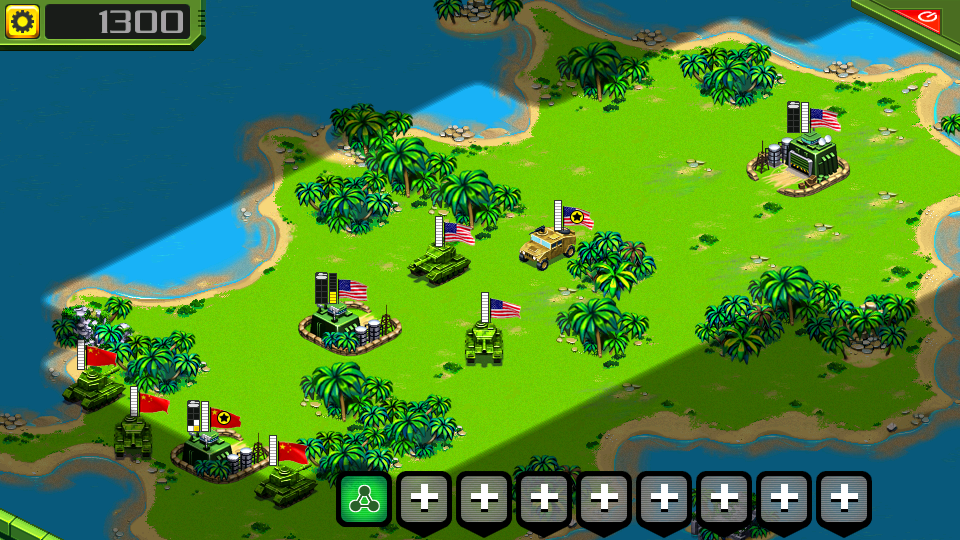
\includegraphics[width=0.8\textwidth]{Images/tropical_storm.png}
  \caption{Tropical Stormfront from Noble Master Games}
  \label{fig:ts}
\end{figure}

Tropical Stormfront was their first release for Android in December 2011 and for iOS in November 2012. It took the RTS experience and simplified it to aim it towards the casual gamers that make up a large percentage of the mobile market. Its simple sprite style isometric graphics, shown in Figure \ref{fig:ts}, are pleasing on the eye and make units and structures easy to identify. The uses of an isometric view also removed the complexity presented by 3D graphics, that could it make it difficult to control, while retaining a well designed style.

The game revolves around a series of short predefined missions. Each mission only takes a matter of minutes to complete and don't really require a huge amount of strategy this caters nicely for the casual gamer. There is also an option for multi-player games with a selection of modes ranging from skirmish to capture the flag, with one user hosting the game. The host is able to choose the game type, map and a number of other options, other users can then join the game.

Unit control for example is cutback, users can control where units should move to as well as which enemies to attack but no other complex commands could be issued. A very useful feature was the ability to group units together and assign said groups to hot-keys along the bottom of the screen. Without these it was difficult to command a number of units in a controlled manor. As well as these assigned groups there was also the option to select units individually, by tapping that unit, or multiple units. Multiple unit selection was handled by tapping the green icon to the left of the hot-key buttons. This then enabled the user to drag over an area units selecting all within that area. It was important for MapWars to retain this level of control while retaining its simplicity. It could even be simplified further by removing manual targeting of enemy units, leaving this up to the games AI system.

Another aspect that is missing is the ability to create and position buildings. Each map comes with a predefined set of bases that can not be altered or moved but enemies can capture other players bases. These bases give players the ability to create new units and are also the mechanism for getting money. New units are built in a fairly standard process of selecting a base which in turn gives a range of units to build. Units cost a certain amount of money or resources to be built and the build process takes an amount of time to complete. After the unit has finished being built it exits the base and can be interacted with as usual. The lack of build queue, in which players can make a list of which units they want built and they will be processed in turn, was found to be restrictive. Inclusion of a build queue seemed plausible while still maintaining the ease of use.

As mentioned previously in game currency is generated based upon the number of bases a player controls. Each base earns \$50 per minute, so the more bases captured the more money earned which in turn allows for building more units. Resource discovery, gathering and management are key aspects on PC based RTS games but could present problems when being implemented on a mobile device. By removing these aspects the developers were able to speed up game play and in turn try to make the game more exciting. Unfortunately the direct correlation between number of units and victory made game play feel predictable as the player who captured the most bases inevitably won.

Tropical Stormfront takes a good approach that, as with a number of the other compromises, directs the game towards casual gamers by removing some of the complex strategy decisions. They focused on fast based game play by setting the player up with a particular scenario with an established base and units with close proximity to the target. MapWars, although sharing many similarities, will ultimately be seeking a different target audience and game play style. The main aspects to be taken forward into the design of MapWars are:
\begin{itemize}
\item Simplify the process of issuing commands to units
\item Ability to select multiple units at once
\item Clutter free UI
\item Cater for the casual gamer while accommodating those who want something more engaging
\item Build queues
\end{itemize}


\section{Objectives}
MapWars is going to attempt to focus on tactical game play with a mobile experience tailored to the users location. All game play will take place on a portion of a world map depending on the players location. While taking as many of the tactical aspects from existing PC RTS games with an elevated focus on resource gathering and long term tactical game play. Unlike some games that allow for fast paced "rushing" (a tactic in which a team will attack an opponent as quickly as possible as to surprise and overwhelm them) MapWars will encourage players to find and gather resources while building a substantial base and selection of units. This is in part due the sparsity of opponents in such a large environment. To try and compensate for the widespread nature of players, as well as the desire to recreate a real world experience, all players will play in a single persistent game. Being persistent all units will be visible even if their respective players are not online increases the emphasis on building a well formed and fortified base.

Problems may be presented with early adopts and those in remote areas who will ultimately not come across other players for considerable portions of their experience. This will undoubtedly lead to players getting bored and leaving the game. To try and combat this possibility game play should try and be enhanced for non-offensive play. The focus on resource gathering, exploration and base development hopefully will be the main combat to this problem, giving players the ability to enjoy the game even without an opponent. Secondly the persistent and location-aware portions will help the game change and evolve as players move around. For example if a player from an unpopulated area spends their time enhancing their units could then travel to a more active area, such as a city, to engage with opponents.

\subsection{Primary Objectives}
The objectives listed are considered to be the minimum required to create a playable game:
\begin{itemize}
\item Ability to authenticate users
\item Display all units on a map centred on the players current location, limited to a given range
\item Location will be determined by all available sensors and the most accurate to be used
\item Appropriate portions of the application will stop functioning when minimized, to preserve battery life and minimize data usage. The application should then return to a playable state when returned to
\item Resource gathering
\item Enable players to create units, within a given range of their current location
\item Enable players to move units, within a given range of their current location
\item Units will engage with enemy that come into range automatically
\end{itemize} 

\subsection{Expanded Objectives}
If the primary objectives are completed before the hand-in date the following objectives will be considered. Each of these extra objectives are not essential to the project but would add extra depth to the game play and ultimately improve the overall experience.
\begin{itemize}
\item Altering the resources generated by each mine based on real world resources in that location
\item Introduction of environment variables such as power requirements. Each structure will add to the energy requirements, if these aren't met the structures will not function.
\item Ability to upgrade units and structures
\item Extra unit and structure types
\item Path finding that follows physical routes e.g. roads utilising a directions API
\item Offline notifications
\end{itemize}


\subsection{Limitations \& Evaluation}
Working with a mobile platform comes with a number of technical challenges and limitations. Most notably is battery life, modern smartphones are capable of a multitude of tasks that increases the demand on the phones battery. This combined with the lightweight, small factor demanded by consumers the battery life is servilely limited. While developing MapWars it was important to keep this in mind and reduce the battery usage where possible. Certain areas that large power savings can be made, such as reducing the use of GPS sensors, can have a detrimental affect on accuracy or responsiveness. For this application the accuracy of the users location as they move around was not of a particular importance as it was used simply to locate them in the game area and not displayed directly. Therefore, with some small experimentation, the frequency in which the location was queried was tweaked to get a satisfactory balance between power usage and accuracy. Redrawing the screen is another drain on the battery so these should be kept to a minimum. The drawback with reducing the number of redraws is the possibility that the on screen movements of units and animations will become jolty and detract from the experience. Again experimenting with the delays within animation threads and reducing unnecessary redraws helps to keep the action smooth.

With over a thousand unique devices each offering a unique subset of sensors, screen sizes and features it is impossible to predict what features will be available on any device that will be running the application. For this reason it was important to take advantage of all possibilities while being aware of the limitations that may be presented. If a device does not support GPS or has it disabled, for example, it was necessary to find an alternative source of location data. Each source of data offered different levels of accuracy so again it was necessary to take this into consideration when determining which source to trust.

The success of this project will be evaluated primarily by it's ability to perform the tasks set out in the main objectives set out earlier in the document. Unit responsiveness when created and moved must be quick and consistent across devices. When a unit is moved on one screen the accuracy in which this is reflected on all other devices within proximity needs to be examined, with the smaller the difference resulting in a positive evaluation. With such a type of game this responsiveness can negate from the users experience and if it's too slow will frustrate and anger the player. Advantage can not be given to users based on their choice of device and connectivity. The applications consideration for the environment, as explained briefly above, is also a critical point to evaluate. As well as just the battery usage of the application the amount of data sent and received also needs to be kept at a minimum.

These objectives are the only the basis and do not give a complete picture of the desired outcome. As well as these objectives the finished application must play well and be a pleasurable experience. These are difficult requirements to quantify and will rely heavily on user testing and feedback. By distributing the application amongst users unfamiliar with any previous incarnations will be the best measure of it's playability. Their ability to play the game without external interaction and their overall enjoyment are the most valuable measurements available.

Previous metrics are focused primarily on the clients representation of data received from the server, the server it self needs to be evaluated. The server is required to be able to handle multiple concurrent connections each issuing commands that may or may not affect the other connected users. It must also be able to control unit movements and automated targeting and attack mechanisms. All while validating users actions and preventing spoofed requests, crafted to give the user an advantage over other users using the Android client.

\chapter{Development Process}
Due to a strict deadline and extensive possibilities the project offered it is important to choose a development life cycle that could both quick and flexible. It needed to be able to allow for rapid development in a controlled manor that would reduce the need for rewriting and refactoring of code. Therefore the methodology will revolve around an iterative life cycle. As the project is easily broken down into a small number of well formed sections these iterations are able to be well formed before development beings.

\section{Introduction}
The development life cycle chosen is that of Rapid Application Development (RAD). This process reduces the need to have a detailed specification or design at the beginning of development. Instead specification, design and implementation are all simultaneous. This life cycle follows more closely to the Spiral Model than that of a more traditional waterfall type life cycle. The Spiral Model, as defined by Barry Boehm\cite{spiral_model}, depicts an evolutionary style of development which still keeps control over the project. Unlike the waterfall model which requires a stringent and detailed design that needs to be followed throughout implementation. Only the highest-priority features are considered for each iteration. The chosen feature is defined, designed and implemented during the cycle. Each cycle results in a prototype of a portion of the final system that can be tested. From this prototype ideas can be tweaked and changed then defined and implemented. Then the next feature can be defined and so on until the desired system is completed.

The RAD life cycle is a further streamlining of the spiral model and only has four distinct stages. Firstly there is the requirements gathering stage where all parties agree on the scope and requirements for the overall project. This is followed by user design where users interact with the developers and create a set of prototypes that are then evaluated by the users. This step is continuous phase that sees the prototypes change and adapt to the users requirements. This phase works in tandem with the construction phase which sees the prototypes be integrated into the final application and tested. With the user still actively involved they can suggest changes and improvements as the application takes shape. After the application is completed the final stage sees its testing, integration and user training.


\section{Modifications}
The spiral and RAD models are defined as an evolutionary method therefore each iteration prototype should be delivered to the stakeholders. These stakeholders can then give their feedback which should be utilized in the next cycle. Seeing as this project does not have any stakeholders this crucial step can not be completed and therefore the model needed to be adapted from a evolutionary to an incremental one. To achieve this the stages were mapped out before implementation began resulting in a slightly increased amount of design. These stages were purposefully left as broad as possible to accommodate necessary changes that would present themselves as development began.

As well as removing the of reworking code by cutting out the feedback loop for each prototype, the user design and construction phases are combined. This single step would see prototypes being worked directly into the current code base. In this way extra development time would not need to be used to integrate the prototype back into the master branch. This combination by itself would slowly reduce the code quality seen across the application as ideas are tested, for this reason spike work is encouraged to be carried out before each iteration. These short spike work sessions should show up any problems and highlight more efficient ways that part of code could be implemented. This will then carry over into the main code when the feature is implemented. It is important to keep this spike work short and focused and full solutions are not the ideal outcome from it.

These modifications were made as a way to streamline development, reducing time spent in design and coding while not reducing code quality or flexibility.




\section{Development Environment}

\subsection{Language}
Developing applications for the Android OS restricts the language choice to just Java combined with an Android framework. This results in code written with Java syntax but are not entirely synonymous with Java. Code is converted from Java Virtual Machine (JVM) compatible code to code that can be run by Dalvik, the vitual machine used by Android. This conversion optimizes the code to be run on devices with limited memory and processing power.

For the server portion of the application it was important to choose a language that would aid in the rapid development methodology outlined for the project. Python is a general purpose high-level programming language that has a relatively small learning curve as well as some personnel background knowledge. It is designed with the express purpose of being highly readable by forcing well formatted code and using English keywords. 

As the chosen hardware for the server is limited in processing power and memory it is important keep overheads to a minimum, which Python does fairly well. If Java had been used a much more powerful server would have been needed to support the same number of processes due to the overheads introduced by the JVM. However there would have been a number of advantages to using the same language as the client. These include a greater understanding of the language as it is used more extensively but more importantly would be code reuse. The client and server both perform many of the same procedures and could have sped up development time and increased accuracy and interoperability as the same packages could have been utilized.

SQLite

\subsection{Development Environment}
It was decided to use the Eclipse IDE as the main editor partly due to it's popularity and abundance of information and also it's improved integration with the SDK. Google provide an Eclipse plugin called Android Development Tools (ADT) which provide a set of tools to streamline the development process. 

Eclipse, sublime, GIT, GitHub, ADB

\subsection{Hardware}
Although the platform has been selected it is also important to examine the target devices.Android has began reaching much wider than just the phone market as it finds its way on to tablets, set-top boxes and netbooks.

Devices? 96\% Android phones, 64\%Table, remaining 20\% netbooks and TVs.

Phones, tablets, broken digitizer

\subsection{Other tools}
DIA?
\chapter{Design}
\section{Overall Architecture}
It was clear from the outset that the server and client portions of the application should be developed independently. The two sections would also be ran independently of each other on different machines. To keep within the time scales of the project only one instance of the server will be running at any time. Multiple servers and load balancing would be ideal but not necessary at this time. The server was written in Python to be run on any compatible server. The client uses Java and designed to run on Android devices, the client then connects directly to the server using PUSH technology.

The client portion was developed by loosely following the wildly acknowledged Model-View-Controller (MVC) architecture. This design was chosen due to it being well known and understood speeding up the process of others understanding the code. Also it's rigid nature should help prevent chaotic and unstructured code. This pattern breaks the code up into three parts: the model which contains the bulk of the application logic; the view which handles changes to UI elements and the controller that handles events and negotiates communication between the model and view.

Nothing radical has been altered about the overall architecture from the progress report. It has simply been expanded while implementing new features.

\section{Class Diagram}
The class diagram for the client portion of the project can be found in Appendix \ref{ap_class}. The supplied class diagram is a simplified representation as it does not include variables or methods. The sheer amount of data was overwhelming when these were included and offered little extra insight into the client architecture. Classes are also not grouped by package as this made the diagram difficult to follow.

The servers architecture is considerably simpler and a diagram is not included in this report.

\section{Use Case Diagram}
\begin{figure}[H]
  \centering
   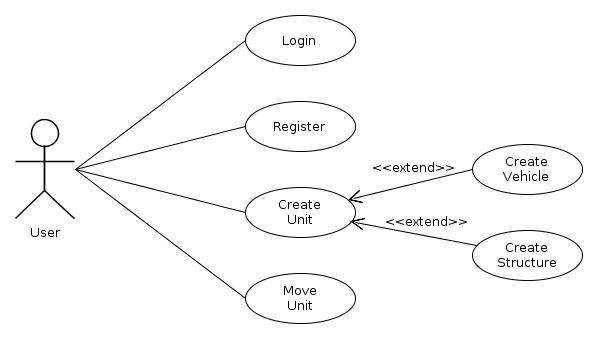
\includegraphics[width=0.8\textwidth]{Images/diagrams/use.png}
  \caption{Use case diagram}
  \label{fig:use}
\end{figure}

All actions that a user can perform are listed on the design user case diagram, Figure \ref{fig:use}. This minimal looking list of actions is all the interaction required from a user. As the more complex behaviours are handled automatically by the server extra actions, such as attack, are not a concern of the user. This harps back to the overall ethos of keeping the game-play simple while retaining the features of a desktop RTS title.




\subsection{Language}
Developing applications for the Android OS restricts the language choice to just Java combined with an Android framework. This results in code written with Java syntax but are not entirely synonymous with Java. Code is converted from Java Virtual Machine (JVM) compatible code to code that can be run by Dalvik, the virtual machine used by Android. This conversion optimizes the code to be run on devices with limited memory and processing power.

For the server portion of the application it was important to choose a language that would aid in the rapid development methodology outlined for the project. Python is a general purpose high-level programming language that has a relatively small learning curve as well as some personnel background knowledge. It is designed with the express purpose of being highly readable by forcing well formatted code and using English keywords. 

As the chosen hardware for the server is limited in processing power and memory it is important keep overheads to a minimum, which Python does fairly well. If Java had been used a much more powerful server would have been needed to support the same number of processes due to the overheads introduced by the JVM. However there would have been a number of advantages to using the same language as the client. These include a greater understanding of the language as it is used more extensively but more importantly would be code reuse. The client and server both perform many of the same procedures and could have sped up development time and increased accuracy and interoperability as the same packages could have been utilized.

The server also required a persistent data store to keep an overview of the users and units between downtime or server migration. The requirements specified matched closely to those given when choosing Python as the programming language. 

\begin{itemize}
\item Non-proprietary
\item Simple, zero-configuration database
\item Relational makes things easy
\item Lightweight
\item Previous knowledge of SQL makes that a preferable language of choice
\item Simple python implementation.
\end{itemize}

A nice looking option was KirbyBase\footnote{http://wiki.python.org/moin/KirbyBase} it matched all of the requirements and being purely python based was a plus. It is a flat-file database so was simple to configure and lightweight, it also had the flexibility of running both as part of an application or in a client-server configuration. Unfortunately development stopped in 2006 and the libraries website has since been taken off-line.

MongoDB\footnote{http://www.mongodb.org/} would have also been a nice solution as it supports a large proportion of the requirements and some other features ideal for this project. Unlike other options it is a NoSQL\footnote{http://www.10gen.com/nosql} database which is an entirely different approach to database design than that of the standard relational database. This would have required considerably more investment of time to learn this new style of working. The main draw to MongoDB is that it offers geospatial indexing and queries. This allows the complex calculations of querying coordinates on a sphere could be handled directly by the DBMS.

The chosen SQLite solution has one long term problem that comes with not being able to run a client-server configuration. Thus restricting the application to a single server. As the popularity and interest in the game increases so would the demand on the server meaning that a more complex, distributed server model would be needed. This is outside of the scope of the current project so this was deemed to be an acceptable compromise.

\section{User Interface}
When developing any application for a small form factor it is important to consider how the user interface can be minimized, and to not clutter the display making precise controls difficult. This is especially important when trying to fit all the functionality of a \gls{rts} game within the small form factor of a mobile device. To get around this problem only the essential controls were included with only a portion of these being accessible from the main game screen.

The main game screen, shown in Figure \ref{fig:isogui}, is entirely taken up by the game map where all unit interaction takes place. Overlaid on this map are the game controls consisting of a control bar (A) and a selection of controls (B). These controls have been minimized to take up as little space as possible while still being accessible and allowing the user the freedom of control desired. Unit manipulation takes place directly on the map itself, units are displayed on a clickable overlay. Selecting a unit is a simple as tapping it, after selecting a unit it can be moved with another single tap in a free area of the map. When a unit becomes selected a health bar is displayed and a estimated attack range. The health bar is also displayed while the unit is under attack.

\begin{figure}[H]
  \centering
   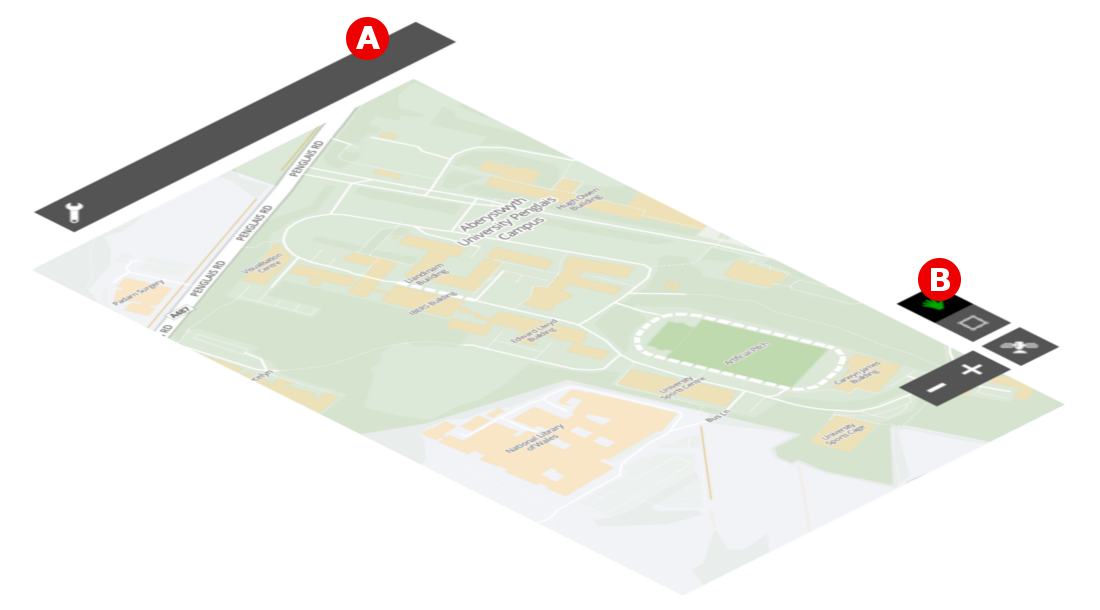
\includegraphics[width=1\textwidth]{Images/layout_include.png}
  \caption{Isometric view of main game screen,\\showing separation between components}
  \label{fig:isogui}
\end{figure}

\chapter{Implementation}


Each iteration of the project will be described




\section{Client Implementation}
\subsection{Mapping}
The first iteration focused on the central component of the application, the map. It was vitally important that an appropriate mapping solution was used.

\subsubsection{Google}
Google provides a simple, easy to use interface to their own maps making it the obvious choice for any Android application. Their maps are accurate, up-to-date and very detailed.

Unfortunately there are a number of restrictions in place stopping their use in a number of situations. The most relevant of which is that they can not be used in an application that is not freely available to the public. Therefore restricting it's use in a paid-for application, such as MapWars may become. As the future of the application is uncertain it seemed desirable to steer clear of as many possible restrictions as possible. For this reason it was important to find a comparable alternative.

\subsubsection{OpenStreet Map}
OpenStreet map is an INSERT DESCRIPTION OF OSM HERE. It's growing popularity means that INSERT STATS ABOUT AREAS COVERED. With an acceptable level of detail combined with it's open SOMETHING(ethos?) made it the next most obvious source.

OSM has an API that allows it to be easily embedded into webpages but no native android SDK. A number of 3rd party libraries are available. The most complete and popular is that provided by MapQuest.

MapQuest are a mapping company that combines proprietary data and OSM data to create their own maps. They offer an Android SDK that gives you the option of which tile source to use. There are obviously restrictions to the proprietary data but if you opt for the free tiles then the same license is used as with OSM. The Android SDK available was designed to mirror the API available for the Google Map SDK. This made swapping out the Google Maps code and replacing it with the MapQuest code was trivial and problem free.

At the point in time of implementing MapQuest the design had called for the option to switch between satellite and road maps. MapQuest's main drawback, and more widely OSM itself, was it's lack of detail. The level of zoom supported was a number of levels less than that of Google Maps. These extra zoom levels would have made unit manipulation easier on smaller devices. Satellite images were the main concern as they were not available at the level of zoom required to make game play comfortable.

MapQuest was used as the mapping solution for a large portion of development and offered a stable platform. Once more of the functionality was in place user testing presented a number of problems with the map tiles being used. Most significant of which was a difficulty in being able to locate units among the details presented with the map. The sprites and colours being used to represent units were experimented with but none were clearly visible. The problem was with the design of the tiles being used and not necessarily the zoom levels present, although this may have helped alleviate the problems.

\subsubsection{MapBox}
One option available was to use a tile creator and host the map tiles on a server. This would be a costly and difficult solution to the problem. Hosting tiles is not a trivial task and require large amounts of storage and bandwidth.

MapBox offer beautiful hosted tiles. They also have their own software called TileMill which allows the creation of bespoke tiles based on any data source which can then be hosted and distributed via their network. TileMill was based on a CSS style syntax allowing you to customise any visual aspect, from line widths, colours, strokes. It also had the ability to import data from any source giving the ability to build up rich tiles with as much detail as required. For MapWars only the most basic detail was required while using a simple colour pallet. The idea was to make any unit stand out against the map while still presenting all the information required to orientate the user with their surroundings. 

Tiles could be loaded from MapBox using a standard URI syntax used by the most tile vendors. This allowed it to integrate easily into any mapping framework.All that was needed was an SDK that allowed custom tile sources. Such functionality was found in OSMDroid. Like with MapQuest, OSMDroid followed the same pattern as Google Maps allowing it to be easily placed into the application without only one substantial problem. OSMDroid was missing one function that was supported by both Google Maps and MapQuest. These function was key in selecting units so had to be reimplemented ... which was not difficult but took time. Assumption was made it would be as effortless as the previous transition. After integration was complete plugging in the URI to my generated tiles was simple and worked straight of the bat.

MapBox did not offer satellite imagery but the beauty and simplicity of the maps being used made up for this. It was also decided that the complexity of such maps would just present the same images as found with the default OSM tiles. Satellite images could always be added to OSMDroid by simply finding a tile source and using that and would have no affect on the functionality of the application. 


\subsection{Location}
Detecting the users location accurately is fundamental and is used directly in controlling game play throughout the game.

There are a number of difficulties presented when trying to accurately determine a users location. Firstly is the array of different sensors available, each with their own unique characteristics, advantages and disadvantages.

When taking location data from a variety of sources it is critical to have a process to determine which is the most accurate to the users current location. Each sensor will gather data at different times and to a different level of accuracy. Whenever this data is processed a judgement needs to be made into whether this is more reliable than the currently known location. This was made based on the following criteria:
- Accuracy
- Age

The accuracy of the users location is not a critical variable within the application as it will not be displayed directly and only to determine the radius of control. Therefore if the location is off by a few hundred meters it will not have a detrimental affect on game play. This allowed all types of sensor to be used, including network estimated location. Network location can be up to asdfoiasjdfiojaoisdfjoasidjfoaisdjf


\subsection{GUI}
9-patch
Different layouts for different devices
Different orientation for different devices


\subsection{Communication}
PUSH/PULL
XML/JSON

\subsection{Units}



\section{Server Implementation}

\subsection{Echo}

\subsection{Units}

\subsection{Storage}

\subsection{AI}

\chapter{Testing}

Detailed descriptions of every test case are definitely not what is required here. What is important is to show that you adopted a sensible strategy that was, in principle, capable of testing the system adequately even if you did not have the time to test the system fully.

Have you tested your system on 'real users'? For example, if your system is supposed to solve a problem for a business, then it would be appropriate to present your approach to involve the users in the testing process and to record the results that you obtained. Depending on the level of detail, it is likely that you would put any detailed results in an appendix.

\section{Overall Approach to Testing}

\section{Automated Testing}

\subsection{Unit Tests}

\subsection{User Interface Testing}

\subsection{Stress Testing}

\subsection{Other types of testing}

\section{Integration Testing}

\section{User Testing}
\chapter{Evaluation}

% Examiners expect to find in your dissertation a section addressing such questions as:

% \begin{itemize}
%    \item Were the requirements correctly identified? 
%    \item Were the design decisions correct?
%    \item Could a more suitable set of tools have been chosen?
%    \item How well did the software meet the needs of those who were expecting to use it?
%    \item How well were any other project aims achieved?
%    \item If you were starting again, what would you do differently?
% \end{itemize}

% Such material is regarded as an important part of the dissertation; it should demonstrate that you are capable not only of carrying out a piece of work but also of thinking critically about how you did it and how you might have done it better. This is seen as an important part of an honours degree. 

% There will be good things and room for improvement with any project. As you write this section, identify and discuss the parts of the work that went well and also consider ways in which the work could be improved. 

% The critical evaluation can sometimes be the weakest aspect of most project dissertations. We will discuss this in a future lecture and there are some additional points raised on the project website. 

While providing a challenging set of targets the final application demonstrated a working prototype of the original concept, creating a multi-player location-aware game for a mobile platform. This was completed while taking into account consideration of the limitations presented by such a platform. A great deal was learnt about both Android development and Python fundamentals.

\section{Primary Objectives}
All primary objectives were at least partially implemented, with most being fully integrated. The only objective not fully covered is the ability to place the running application in the background and then restore it.

User accounts, both registration and authentication, are implemented on both the server and client. User accounts are persistently stored on the server-side, while session based authentication is used to keep track of connected clients.

The ability to create units is fully functional, with these actions being quickly reflected on other players devices. Players can then select their units and instruct them to move to a new location. With two modes available to select units this processes is simple and flexible. Units will then start travelling towards the target location, again with other players devices displaying these updates accurately. Units automatically engage with enemy units as they come into range with dynamic consequences.

A simplified form of resource gathering was adopted taking inspiration from Tropical Stormfront's model. Placing of mines automatically gathered a fixed amount resources at regular intervals. Although not being the intended solution it was a satisfactory compromise to get the functionality in place on time.

\section{Expanded Objectives}
Unfortunately none of the secondary objectives were reached due to the time scale of the project. Some of these objectives would be fairly trivial to implement but were decided to be left out for the sake of improving the fundamental objectives.

Adding additional units and structure types with individual characteristics would be the easiest of these to add and would require minimal alterations to both the client and server. Removing hard coded characteristics in favour of inherited values from a list of available types. Once these alterations were made it would then be possible to add any amount of different types without altering the underlying code. Likewise upgradable units and structures and environment variables would have required a similar amount of investment.

Offline notifications would also have been possible using Google's cloud messaging (GCM) service\cite{gcm}. This service allows data to be transmitted to Android devices via Google's servers. Data is limited to a 4kb payload so would most likely have been a simple notification message. This message could then be disabled to the user from which they can decide whether to open the MapWars application and respond or ignore it. The nice feature of GCM is that messages are delivered to applications even if they are closed, therefore allowing for notifications to be displayed when the application is not in use. This would be an important feature in a release version, increasing user retention, but for this prototype it was not an integral part.

The other secondary objectives were far more ambitious. The data is widely available for both the path finding and variable resources ideas but incorporating these into the project would be more difficult. MapQuest, for example, offer a limit-free open directions API\cite{mapquest_directions} from which it is possible to get a series of way points. These coordinates represent the route between two supplied locations. Unfortunately mapping these to unit movements would have required a considerable amount of investment in both the client and server portions of the application. 

\section{Critical Evaluation}
Retrospectively the initial objectives were more optimistic than first imagined. That being said they were necessary to get a full experience of what such a game would require. The overall result was a playable prototype that gave a feel as to what a completed version would be like. It was encouraging to see that there were no major complications during development and the result was an enjoyable experience to play.

A major area in which this project is lacking is in comprehensive testing. This is proof of the difficulty of maintaining a consistent approach across a development life cycle. Testing should have been an integral part of each iteration cycle, unfortunately this was not followed as rigorously as it should have been. This can be entirely blamed on the developer wanting to focus more attention on completing functional aspects of the code rather than testing. The availability and domain knowledge of JUnit would have made this a not to difficult task and may have, unnoticed by the developer, in creased productivity and accuracy. That being said no major problems were en-counted directly related to the lack of such testing. This could be attributed to the nature of the application which requires a fair amount of observational testing during development; helping spot any errors quickly.


\subsection{Known Bugs}
Current path finding techniques on the server-side are rudimentary. Although fulfilling the requirement of moving a unit from point A to point B it does so in a straight line, not taking other units into account. This simplistic approach leads to units manoeuvring directly over the top of other units. No obvious solution, within the currently implemented process, was found to prevent this. It would have been possible to create way points the unit could follow that would create a non-linear path. This would avoid static obstacles but could not predict the movement of other units. To effectively avoid moving units a more sophisticated intelligent system would need to be devised as well as an increase in server-client communication.

This path finding also leads to another bug which is most apparent when two units are selected at the same time and directed to the same location. The two units will reach the end location and position themselves in the same location. At this point it will become impossible to select just one of these units as they occupy the same space. Resulting in two units merging into one without the ability to separate them. A solution could be imagined where when the server receives a request to move a unit into a location; this location is then checked against other units positions and target positions. If this request matches with another unit the target location will be modified. So that the unit comes to rest as close to the target location while not impeding on any other units.


Inconsistency when placed in background

\subsection{Improvements}
Due the time frame available a number of features, as mentioned before, were not implemented. By implementing these expanded objectives the overall game-play could be improved.

Fixing the known bugs would be a high priority, especially the ability to place the running application in the background while keeping sync with the server. This is expected to be a natural behaviour of the end user and would lead to frustration if presented in its current form.

The graphics within the Android client require more work as they are currently flat images. Adding in animation of units and scenery as well as visualizing attacks would add a lot to the experience.

Reworking the server architecture to be scalable and work across multiple servers would be necessary before release. These alterations would see the server being able to hand much larger amounts of traffic. It would be desirable to create a transparent proxy that routed connections to one of a number of servers, each running independently of the others. These servers would simply handle updates and responses and would delegate the AI portion of functionality to a separate machine. To make all this possible a different DBMS would be required to allow multiple connections from different servers, this would be running on a dedicated machine.


\section{Summary}
It is enjoyable and this type of game could be viable for mobile devices.


% add any additional chapters here

\setemptyheader
\addcontentsline{toc}{chapter}{Appendices}
\chapter*{Appendices}
\pagebreak

\fancypagestyle{plain}{%
%\fancyhf{} % clear all header and footer fields
\fancyhead[L]{\textsl{Appendix\ \thechapter}}
\fancyhead[R]{\textsl{\leftmark}}}

\appendix
\fancyhead[L]{\textsl{Appendix\ \thechapter}}
\fancyhead[R]{\textsl{\leftmark}}
\fancyhead[C]{}
\fancyfoot[C]{\thepage}
\renewcommand{\headrulewidth}{0.4pt}
\renewcommand{\chaptermark}[1]{\markboth{#1}{}}

\fancyhead[L]{\textsl{Appendix\ \thechapter}}
\fancyhead[R]{\textsl{\leftmark}}
\fancyfoot[C]{{\thepage} of \pageref{LastPage}}

\chapter{Third-Party Code and Libraries}

If you have made use of any third party code or software libraries, i.e. any code that you have not designed and written yourself, then you must include this appendix. 

As has been said in lectures, it is acceptable and likely that you will make use of third-party code and software libraries. The key requirement is that we understand what is your original work and what work is based on that of other people. 

Therefore, you need to clearly state what you have used and where the original material can be found. Also, if you have made any changes to the original versions, you must explain what you have changed. 


\chapter{Class diagram}\label{ap_class}

\begin{figure}[H]
  \centering
  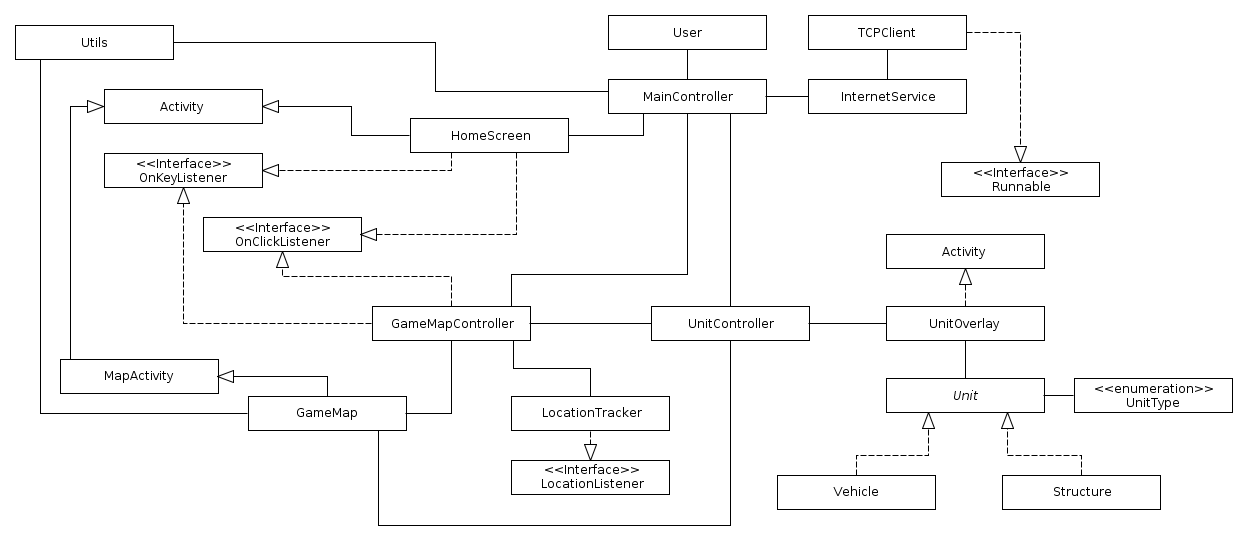
\includegraphics[height=0.3\textheight, angle=90]{Images/diagrams/class.png}
\end{figure}



\chapter{Server Testing Data Generator}\label{server_testing}

\begin{verbatim}
#!/usr/bin/env python
import socket
import sys
import time
import re
import json


HOST = 'localhost'
PORT = 4565

sess = None
userID = None

try:
  sock = socket.socket(socket.AF_INET, socket.SOCK_STREAM)
  sock.connect((HOST, PORT))
except socket.error, msg:
  sys.stderr.write("[ERROR] %s\n" % msg[1])
  sys.exit(1)


while True:
  n = raw_input("> ")

  msgDic = dict()

  if n == "exit":
    break  # stops the loop
  else:
    match = re.findall("[^\s]+", n, re.M|re.I)
    if match:
      if match[0] == 'login':
        msgDic['action'] = "user.login"
        msgDic['user'] = match[1]
        msgDic['pass'] = match[2]
      elif match[0] == 'register':
        msgDic['action'] = "user.register"
        msgDic['user'] = match[1]
        msgDic['pass'] = match[2]
        msgDic['email'] = match[3]
      elif match[0] == 'location':
        msgDic['action'] = "user.location"

        if len(match) == 3:
          msgDic['lat'] = match[1]
          msgDic['lon'] = match[2]
        else:
          msgDic['lat'] = '52.35184333541474'
          msgDic['lon'] = '-1.966477632522583'
      elif match[0] == 'unit':
        msgDic['action'] = "unit.create"
        msgDic['type'] = match[1]
        msgDic['lat'] = match[2]
        msgDic['lon'] = match[3]
      elif match[0] == 'move':
        msgDic['action'] = "unit.move"
        msgDic['id'] = match[1]
        msgDic['lat'] = match[2]
        msgDic['lon'] = match[3]
      else:
        continue
      
      if sess:
        msgDic['sess'] = sess
      if userID:
        msgDic['userID'] = userID

      msg = json.dumps(msgDic)
      print '\x1b[38;5;15m' + "S " + msg + '\033[0m'
      sock.send(msg)


    else:
      continue


  rec = sock.recv(2048)
  try:
    data = json.loads(rec)

    #check for session data
    if data['action'] == 'user.login' and data['status'] == 1:
      sess = data['sess']
      #sess = 'cat'
      userID = data['userID']

    if data['status'] == 1:
      print '\x1b[38;5;46m' + "R " + rec + '\033[0m'
    else:
      print '\x1b[38;5;160m' + "R " + rec + '\033[0m'
  except ValueError:
    print rec


sock.close()

sys.exit(0)

\end{verbatim}

\fancypagestyle{plain}{%
   \fancyhead{} %[C]{Annotated Bibliography}
   \fancyfoot[C]{{\thepage} of \pageref{LastPage}} % except the center
   \renewcommand{\headrulewidth}{0pt}
   \renewcommand{\footrulewidth}{0pt}
}

\setemptyheader

\nocite{*} % include everything from the bibliography, irrespective of whether it has been referenced.

% the following line is included so that the bibliography is also shown in the table of contents. There is the possibility that this is added to the previous page for the bibliography. To address this, a newline is added so that it appears on the first page for the bibliography. 
\addcontentsline{toc}{chapter}{Annotated Bibliography} % Adds References to contents page

%
% example of including an annotated bibliography. The current style is an author date one. If you want to change, comment out the line and uncomment the subsequent line. You should also modify the packages included at the top (see the notes earlier in the file) and then trash your aux files and re-run. 
%\bibliographystyle{authordate2annot}
\bibliographystyle{IEEEannot}
\renewcommand{\bibname}{Annotated Bibliography} 
\bibliography{References/references} % References file


\end{document}
